\section{face-onとedge-onの導出}
図\ref{fig:faceon,edge-on}のように、銀河の回転面の上方または下方から見ているとき、その銀河をface-on galaxyと呼び、銀河の回転面を横から見ているとき、その銀河をedge-on galaxyという。シミュレーション上に作られた銀河は任意の方向から見ることができ、回転も自由に行うことができる。

\begin{figure}[htbp]
	\centering
	\begin{minipage}[b]{0.48\linewidth}
		\centering
		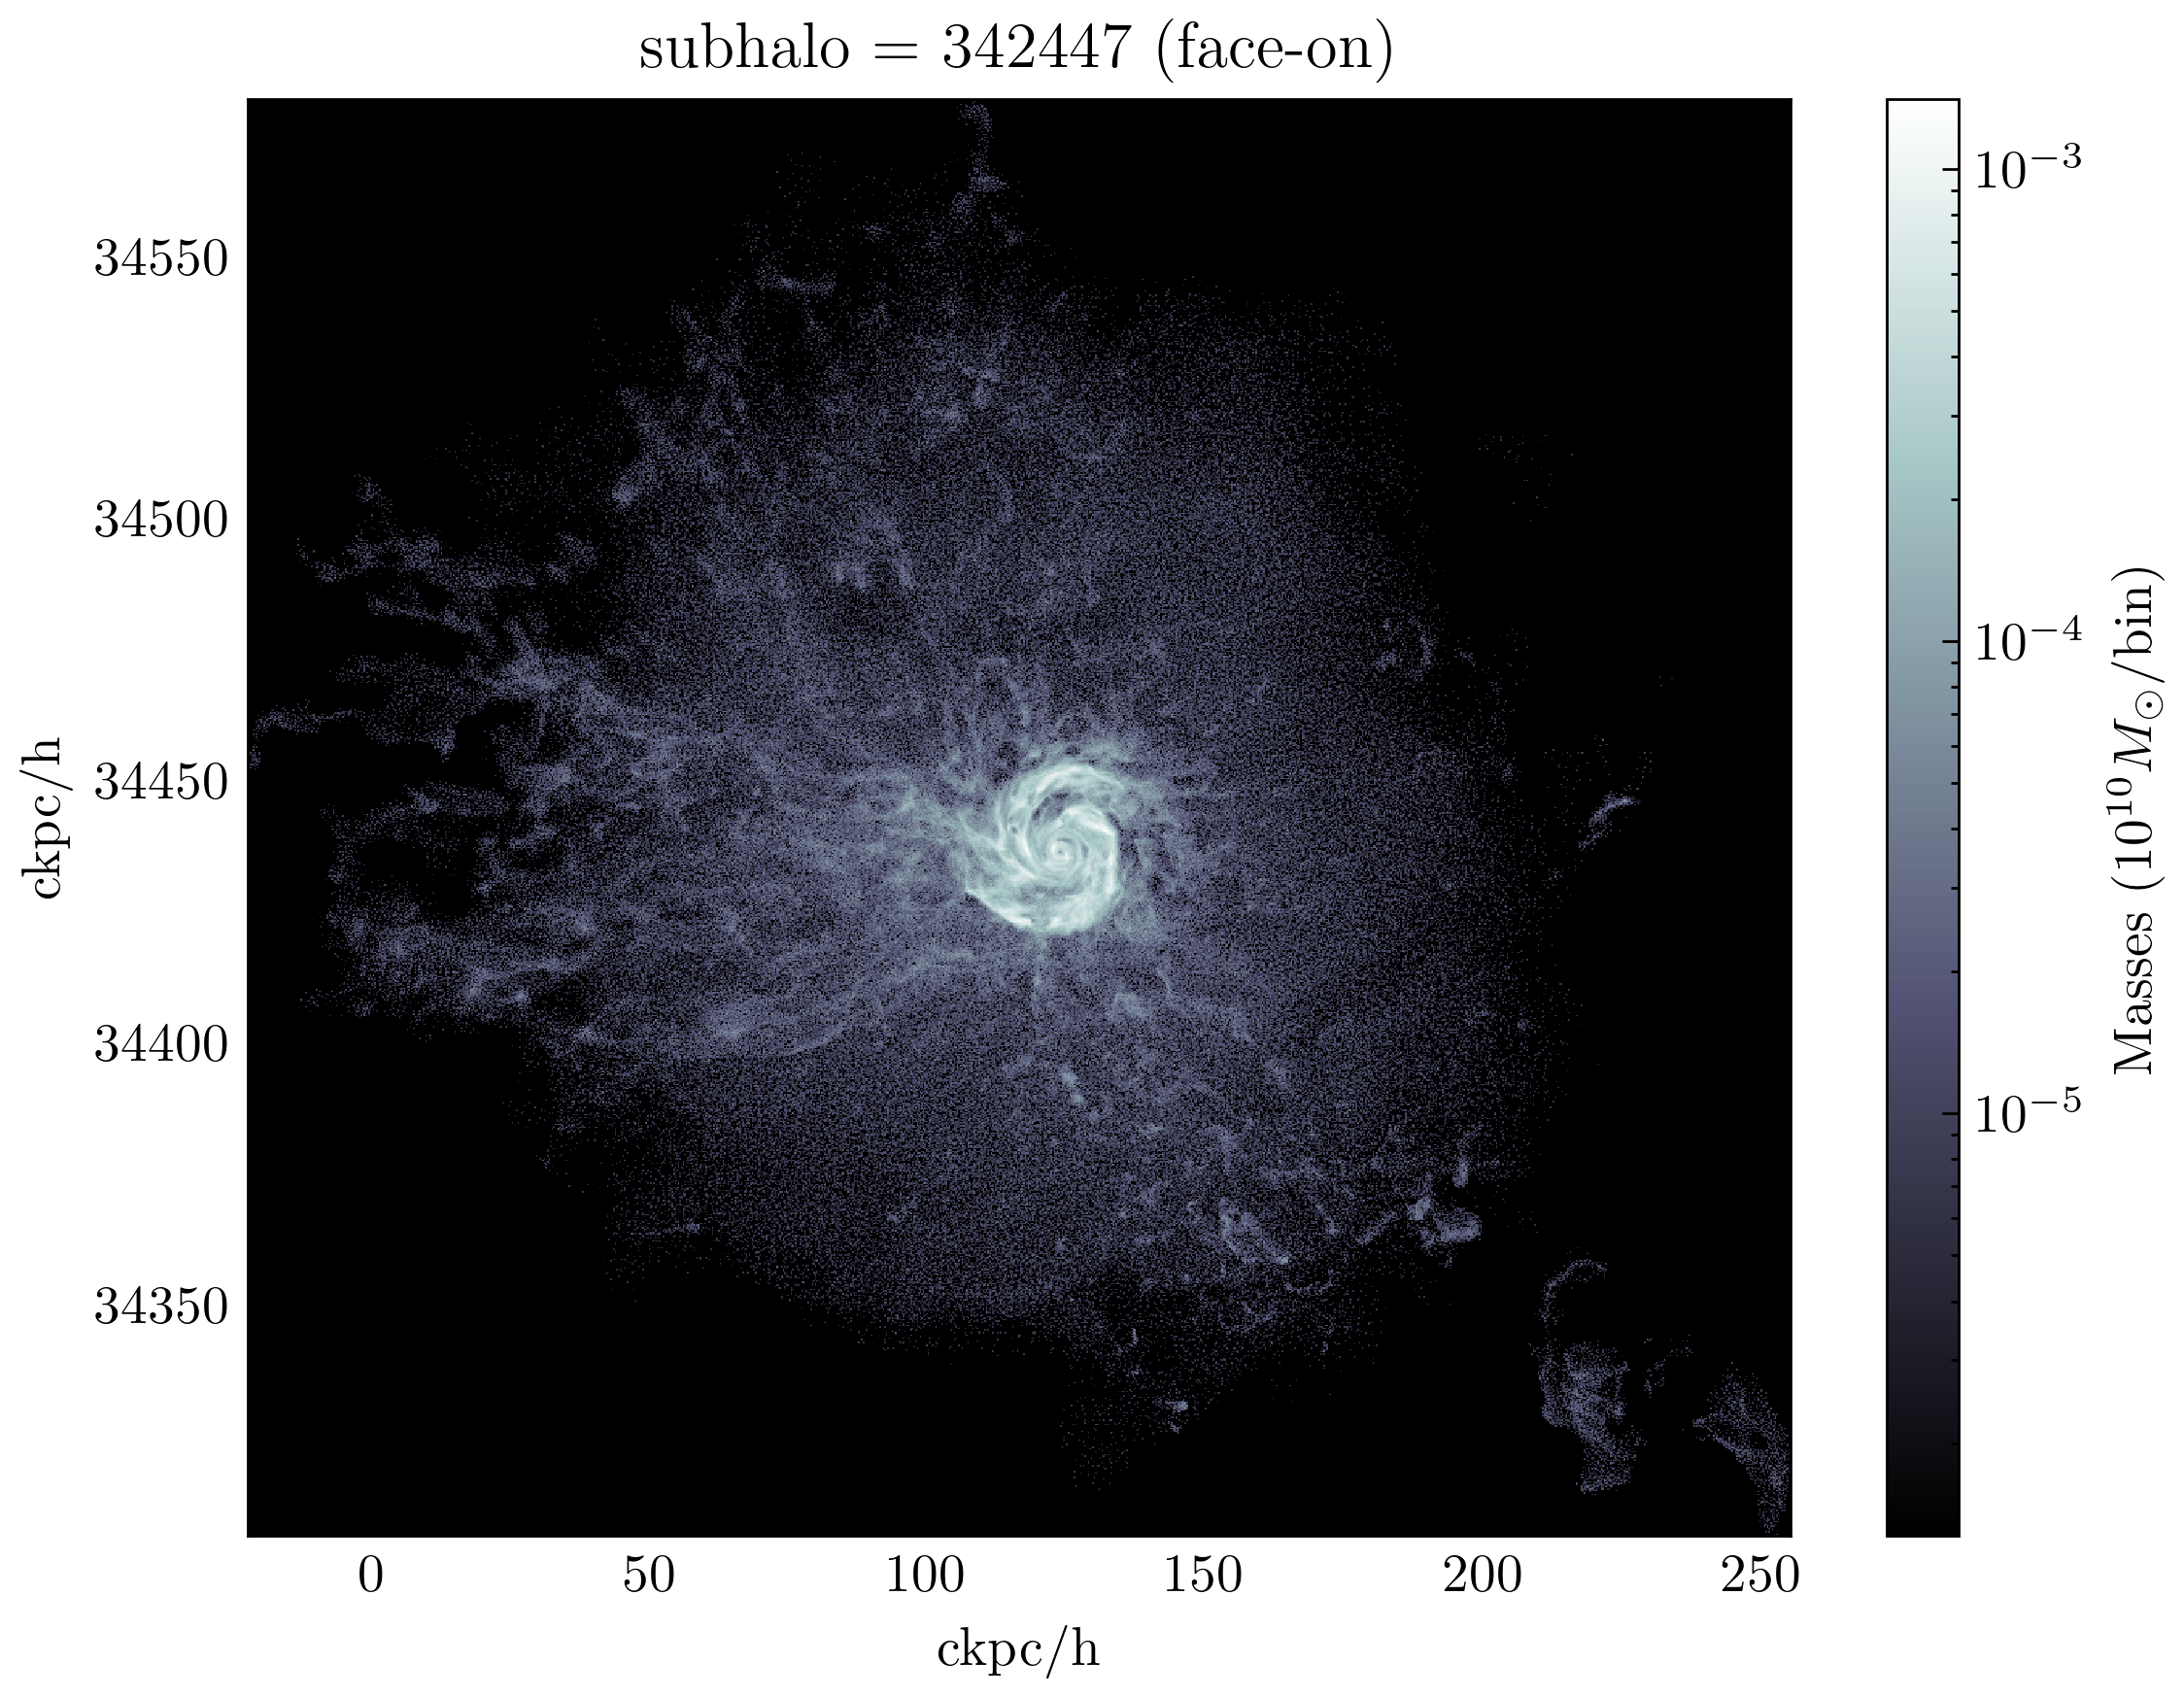
\includegraphics[width=\linewidth]{./pic/face-on}
	\end{minipage}
	\begin{minipage}[b]{0.48\linewidth}
		\centering
		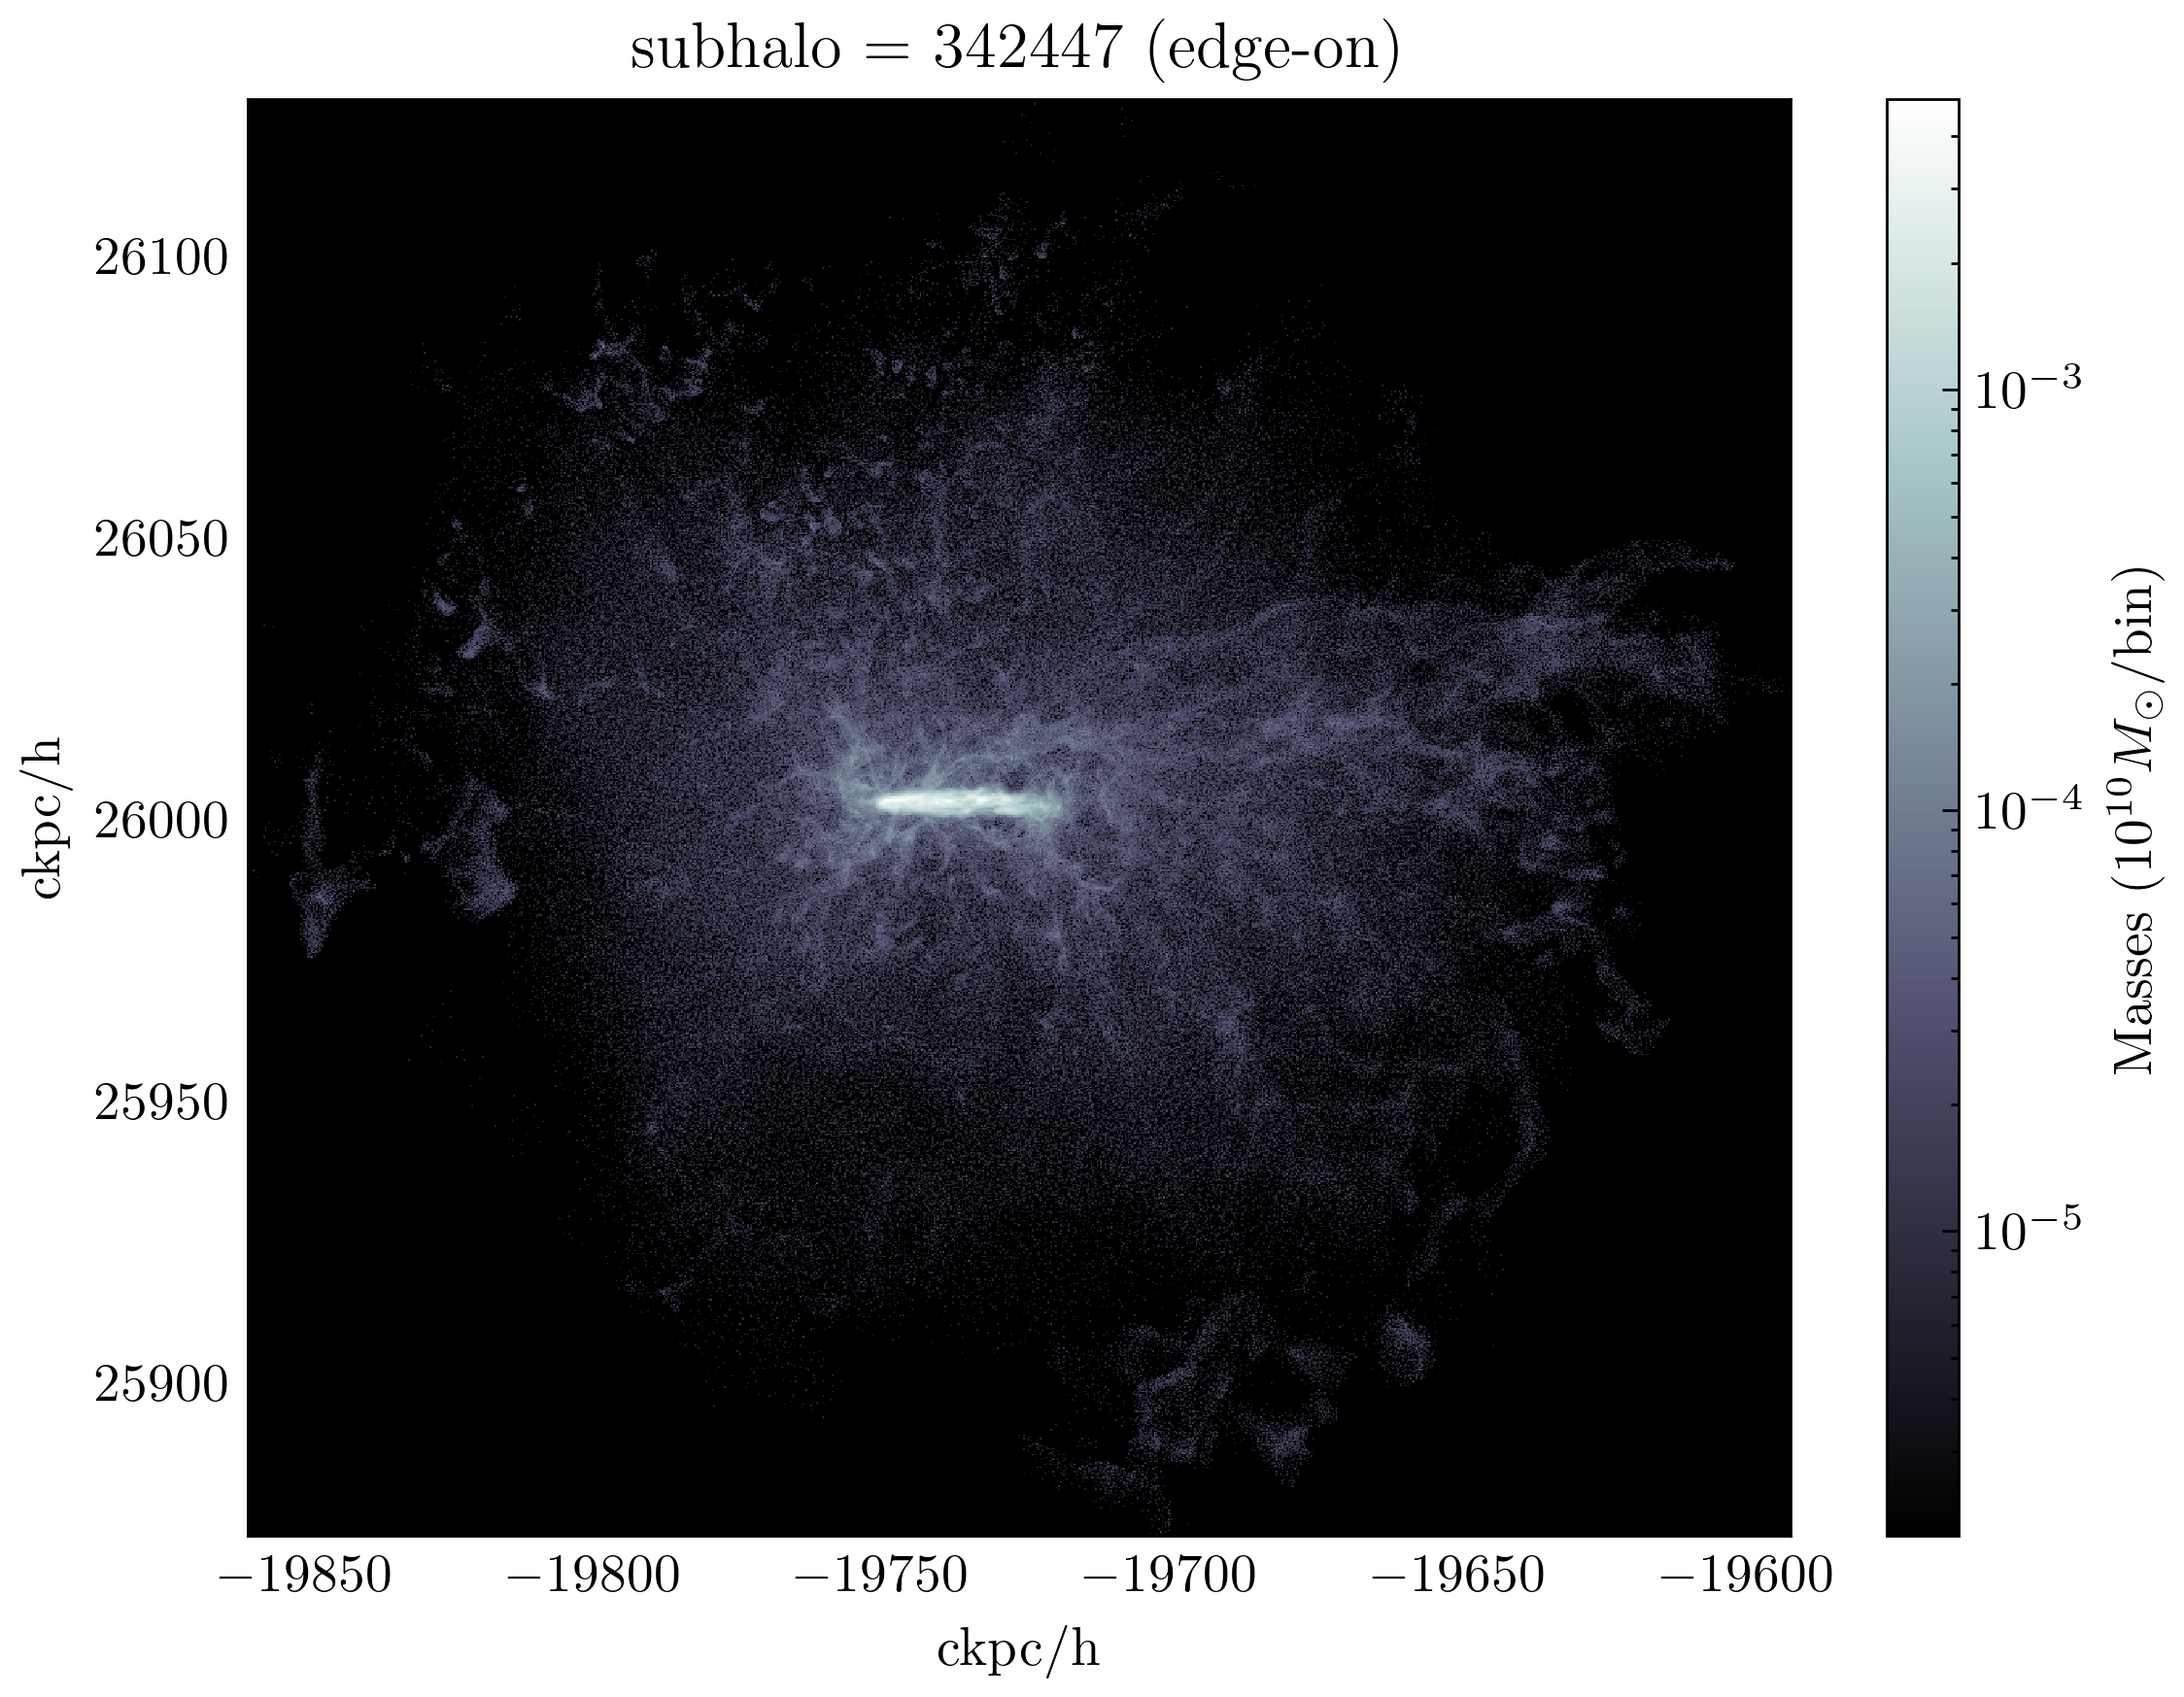
\includegraphics[width=\linewidth]{./pic/edge-on}
	\end{minipage}
	\caption{}
	\label{fig:faceon,edge-on}
\end{figure}

face-onの方向は質量分布が最も安定する方向と見ることもでき、その向きへの回転行列は次のように計算を行うことができる。粒子$i$の座標・質量を添字$i$を用いて慣性モーメントテンソル$I$は
\begin{align}
	I = \sum_{i} \begin{pmatrix}
		m_i (y_i^2 + z_i^2) & -m_iy_ix_i & -m_iz_ix_i \\
		-m_i x_i y_i & m_i (x_i^2 + z_i^2) & -m_i z_iy_i \\
		-m_i x_i z_i & -m_i y_i z_i & m_i (x_i^2 + y_i^2)
	\end{pmatrix}
\end{align}
で与えられる。慣性モーメント$I$の固有値$\lambda_j$ (ただし $\lambda_0 < \lambda_1 < \lambda_2$)、固有ベクトル$\bm{\chi}_j \ (j = 0,1,2)$を求めると、回転行列は$[ \bm{\chi}_0, \bm{\chi}_1, \bm{\chi}_2 ]$となる。またedge-onはさらに$x$軸に対して$\ang{90}$回転すればよい。